\documentclass[sigconf,natbib=false]{acmart}
%%%%%%%%
% Packages
%%%%%%%%

\usepackage[backend=bibtex]{biblatex}

% Filter warnings issued by package biblatex starting with "Patching footnotes failed"
% Source: https://tex.stackexchange.com/questions/202988/beamer-patching-footnotes-warning-patching-footnotes-failed-footnote-detectio
\usepackage{silence}
\WarningFilter{biblatex}{Patching footnotes failed}

% For formal tables
\usepackage{booktabs} 
\usepackage{hyperref}
\usepackage{cleveref}

\usepackage{csquotes}

%%%%%%%%
% Remove copyright
%%%%%%%%
\setcopyright{none}
\settopmatter{printacmref=false}
\acmISBN{} % set this to remove ISBN
\acmDOI{} % set this to remove DOI

\newcommand{\burl}[1]{\textbf{\url{#1}}}

%%%%%%%%
% Meta information
%%%%%%%%
\acmConference[]
	{Masterpraktikum Lehrstuhl X}
	{SoSe \the\year}


%%%%%%%%
% Bibliography sources
%%%%%%%%

% * you can use a remote bibliography from BibSonomy (change 'dmir' to your own username)
%\addbibresource[location=remote]{http://www.bibsonomy.org/bib/user/dmir/myown}

% * or a local file
\addbibresource{bibliography.bib}



\begin{document}

%%%%%%%%
% Front matter
%%%%%%%%

\title{Bericht Masterpraktikum}
%\subtitle{An optional subtitle}

\author{Armin Bernstetter}
\affiliation{%
  \institution{University of W\"urzburg}
  \today
}
% \email{trovato@corporation.com}


\begin{abstract}
This report is a summary of the 
\end{abstract}


%%%%%%%%
% Content
%%%%%%%%

\maketitle

\section{Introduction/Motivation}

The general task of this project was to expand a corpus of german text and then train language models on this corpus.

This was based on the success of OpenAI's GPT-2 project which trained a language model on 40gb of english web text. The model was so successful in tasks such as text generation that OpenAI refused to release the training code and the entire model out of ethical reasons. The concern was that malicious parties could use GPT-2 to generate e.g. fake news for their own good.


\section{Crawler}

Several available german text corpora were already included in the existing corpus. This included the german Wikipedia and novels. 

Crawling the web or rather specific pages for german text is a good way to get new text data.


\paragraph{Reddit}
Pages that were considered initially were german subreddits on Reddit. This includes subreddits such as \textbf{reddit.com/r/de} or \textbf{reddit.com/r/de\_iama}. Reddit's API unfortunately limits the amount of requests a script can make and would have required a workaround repeatedly requesting new tokens etc.

For future work it could make sense to look into \url{https://pushshift.io/} which offers a number of Reddit data dumps, mostly from some years ago.

\paragraph{Wattpad}

Another page that was considered briefly was Wattpad \url{https://www.wattpad.com/}, a \enquote{social storytelling} platform. Users can share their own stories there and read those of other users. Upon examination of the web page's structure and HTML code it was decided that Wattpad obviously are not keen on users crawling their site. Therefore Wattpad was dismissed as well.

\paragraph{Team Andro} The website Team Andro \url{https://www.team-andro.com/} is a german Bodybuilding and weightlifting board. It contains articles on training, nutrition, sport events and more. More importantly, however, it is accompanied by a large german web forum with a user count of almost 300.000 and around 10 million forum posts in total (last checked 2019-09-25).

Upon inquiry the site administrator provided some helpful advice and a link to Team-Andro's sitemap which allowed to iterate through most of the forum's publicly available HTML pages.

These pages were then parsed from HTML and saved in a directory structure representing the forum structure of Team Andro with each post represented as one text file. Additionally, meta data such as user names, time stamps etc were saved in a mongoDB database.


\section{The Dataset}

Prior to the addition of the Team-Andro text data, the existing corpus consisted of a collection of various german text sources. This corpus contains for example the german Wikipedia and german novels and in total amounted to around 8GB of plain text files


The Team-Andro corpus consists of mostly german web text. As such it is often unstructured, meaningless text without contiguous sentences. It is not as \enquote{bad} as e.g. Twitch text but still contains its fair share of internet slang and site-internal phrases and memes.

Phrases which are extremely overrepresented are for example \enquote{\textit{[username] hat am [date] geschrieben:}}.
This indicates a quote of an earlier post inside a new post which often results in repetitions and nested posts.

Additionally to a corpus with a directory structure representing the forum structure, the Team-Andro text was also merged into simple text files with 50MB each. This corpus consists of 2.8GB of plain text files.



\section{ELMo}
\cite{Peters:2018}

\begin{itemize}
	\item Visualisierte elmo embeddings? TODO
\end{itemize}

\section{GPT-2}
After failing to actually work with the ELMo embeddings for text generation, priorities were set more towards GPT-2 which had been the initial goal of the project.



\cite{radford2019language}

Github user \enquote{nshepperd} created a fork of GPT-2 containing Python scripts to train a GPT-2 model. This code was successfully used by blogger and author \enquote{Gwern} (\url{https://www.gwern.net}) to train a GPT-2 model for creating poetry.

As a side note, Reddit user \burl{https://www.reddit.com/u/disumbrationist} created a subreddit used solely by bots of various subreddits trained using \textit{nshepperd's} code. This subreddit can be found at \burl{https://www.reddit.com/r/SubSimulatorGPT2/}.

Another fork/implementation that was considered for training was created by github user ConnorJL \burl{https://github.com/ConnorJL/GPT2}. At the time (July/August 2019), ConnorJL's code was not usable due to some issues with their files uploaded to Google storage.

At the time of writing this report (\today), these issues seem to have been resolved and the repository received some updates in early September. See  also future work in \cref{sec:FW}.


At the time of training, OpenAI had released a small (124M parameters) and a medium (355M parameters) model. To compare the differences in the quality of the generated text, two models were trained.

One was trained on top of the pre-trained 124M model and used a very small sample size of the text data (two 50MB files, one from Team-Andro, the other from the existing corpus).

The second model was trained using the 355M model and the entire corpus. 

Both models were trained for around two weeks. The small model managed to do 522.000 steps, the larger one 180.000 steps.


Unfortunately until the very end it was not possible to determine how much actual text the models had seen at any given training step. Nshepperd's code was rather opaque in this regard.


\begin{itemize}
	\item Welche implementierung und warum?
	\item der blog post mit den gedichten
	\item welche modelle kamen raus
	\item Fragen und Zweifel/Probleme. Undurchsichtige Trainingsskripte usw
	\item sample output und interactive prompt samples
\end{itemize}



\section{What could have gone better?/Future Work}
\label{sec:FW}
Many problems during this project, especially with training the language models, arose because of the choice to use existing code. Trying to understand e.g. nsheppard's code took a surprising amount of time. Time, which might have even been used to write own data loaders and training scripts for GPT-2.

On the other hand, ConnorJL's GPT-2 implementation was updated recently and some issues fixed. It might be worth it to have another look at this before trying to write custom training scripts.

Since the ELMo training was abandoned rather early during this project in favor of GPT-2, it was not possible to look into what to actually do with the trained ELMo embeddings. I did not manage to find out how to use ELMo for text generation.




 
%\section{Introduction}
The introduction.
%\section{The Body of The Paper}
Typically, the body of a paper is organized into a hierarchical
structure, with numbered or unnumbered headings for sections,
subsections, sub-subsections, and even smaller sections.  The command
\texttt{{\char'134}section} that precedes this paragraph is part of
such a hierarchy.\footnote{This is a footnote.} \LaTeX\ handles the
numbering and placement of these headings for you, when you use the
appropriate heading commands around the titles of the headings.  If
you want a sub-subsection or smaller part to be unnumbered in your
output, simply append an asterisk to the command name.  Examples of
both numbered and unnumbered headings will appear throughout the
balance of this sample document.

Because the entire article is contained in the \textbf{document}
environment, you can indicate the start of a new paragraph with a
blank line in your input file; that is why this sentence forms a
separate paragraph.

\subsection{Type Changes and {\itshape Special} Characters}

We have already seen several typeface changes in this sample.  You can
indicate italicized words or phrases in your text with the command
\texttt{{\char'134}textit}; emboldening with the command
\texttt{{\char'134}textbf} and typewriter-style (for instance, for
computer code) with \texttt{{\char'134}texttt}.  But remember, you do
not have to indicate typestyle changes when such changes are part of
the \textit{structural} elements of your article; for instance, the
heading of this subsection will be in a sans serif\footnote{Another
  footnote here.  Let's make this a rather long one to see how it
  looks.} typeface, but that is handled by the document class file.
Take care with the use of\footnote{Another footnote.}  the
curly braces in typeface changes; they mark the beginning and end of
the text that is to be in the different typeface.

You can use whatever symbols, accented characters, or non-English
characters you need anywhere in your document; you can find a complete
list of what is availablevia your favorite search engine.

\subsection{Math Equations}
You may want to display math equations in three distinct styles:
inline, numbered or non-numbered display.  Each of
the three are discussed in the next sections.

\subsubsection{Inline (In-text) Equations}
A formula that appears in the running text is called an
inline or in-text formula.  It is produced by the
\textbf{math} environment, which can be
invoked with the usual \texttt{{\char'134}begin\,\ldots{\char'134}end}
construction or with the short form \texttt{\$\,\ldots\$}. You
can use any of the symbols and structures,
from $\alpha$ to $\omega$.
This section will simply show a
few examples of in-text equations in context. Notice how
this equation:
\begin{math}
  \lim_{n\rightarrow \infty}x=0
\end{math},
set here in in-line math style, looks slightly different when
set in display style.  (See next section).

\subsubsection{Display Equations}
A numbered display equation---one set off by vertical space from the
text and centered horizontally---is produced by the \textbf{equation}
environment. An unnumbered display equation is produced by the
\textbf{displaymath} environment.

Again, in either environment, you can use any of the symbols
and structures available in \LaTeX\@; this section will just
give a couple of examples of display equations in context.
First, consider the equation, shown as an inline equation above:
\begin{equation}
  \lim_{n\rightarrow \infty}x=0
\end{equation}
Notice how it is formatted somewhat differently in
the \textbf{displaymath}
environment.  Now, we'll enter an unnumbered equation:
\begin{displaymath}
  \sum_{i=0}^{\infty} x + 1
\end{displaymath}
and follow it with another numbered equation:
\begin{equation}
  \sum_{i=0}^{\infty}x_i=\int_{0}^{\pi+2} f
\end{equation}
just to demonstrate \LaTeX's able handling of numbering.

\subsection{Citations}
Here are some citations: 
\cite{becker2017mixedtrails,Ring2017,kass1995bayes}.
We use BibLatex\footnote{\url{https://ctan.org/pkg/biblatex}} to create citations.
This allows to load citations from a file (e.g. \texttt{bibliography.bib}) or directly from BibSonomy\footnote{\url{https://www.bibsonomy.org}}. 
See the source code for examples.

Run pdflatex, then biber, then pdflatex twice (to resolve references)
to create the \texttt{.bbl} file.  

\subsection{Tables}
Because tables cannot be split across pages, the best
placement for them is typically the top of the page
nearest their initial cite.  To
ensure this proper ``floating'' placement of tables, use the
environment \textbf{table} to enclose the table's contents and
the table caption.  The contents of the table itself must go
in the \textbf{tabular} environment, to
be aligned properly in rows and columns, with the desired
horizontal and vertical rules.  Again, detailed instructions
on \textbf{tabular} material
are found in the \textit{\LaTeX\ User's Guide}.

Immediately following this sentence is the point at which
Table~\ref{tab:freq} is included in the input file; compare the
placement of the table here with the table in the printed
output of this document.

\begin{table}
  \caption{Frequency of Special Characters}
  \label{tab:freq}
  \begin{tabular}{ccl}
    \toprule
    Non-English or Math&Frequency&Comments\\
    \midrule
    \O & 1 in 1,000& For Swedish names\\
    $\pi$ & 1 in 5& Common in math\\
    \$ & 4 in 5 & Used in business\\
    $\Psi^2_1$ & 1 in 40,000& Unexplained usage\\
  \bottomrule
\end{tabular}
\end{table}

To set a wider table, which takes up the whole width of the page's
live area, use the environment \textbf{table*} to enclose the table's
contents and the table caption.  As with a single-column table, this
wide table will ``float'' to a location deemed more desirable.
Immediately following this sentence is the point at which
Table~\ref{tab:commands} is included in the input file; again, it is
instructive to compare the placement of the table here with the table
in the printed output of this document.


\begin{table*}
  \caption{Some Typical Commands}
  \label{tab:commands}
  \begin{tabular}{ccl}
    \toprule
    Command &A Number & Comments\\
    \midrule
    \texttt{{\char'134}author} & 100& Author \\
    \texttt{{\char'134}table}& 300 & For tables\\
    \texttt{{\char'134}table*}& 400& For wider tables\\
    \bottomrule
  \end{tabular}
\end{table*}
% end the environment with {table*}, NOTE not {table}!

It is strongly recommended to use the package booktabs\footnote{\url{https://ctan.org/pkg/booktabs}}
and follow its main principles of typography with respect to tables:
\begin{enumerate}
\item Never, ever use vertical rules.
\item Never use double rules.
\end{enumerate}
It is also a good idea not to overuse horizontal rules.


\subsection{Figures}

Like tables, figures cannot be split across pages; the best placement
for them is typically the top or the bottom of the page nearest their
initial cite.  To ensure this proper ``floating'' placement of
figures, use the environment \textbf{figure} to enclose the figure and
its caption.

This sample document contains examples of \texttt{.png} files to be
displayable with \LaTeX.  
For this to work you should use PdfLatex.
You can also include files in the
\texttt{.pdf} format.  

\begin{figure}

\includegraphics{res/cats}
\caption{A sample black and white graphic.}
\end{figure}

\begin{figure}

\includegraphics[height=1in, width=1in]{res/cats}
\caption{A sample black and white graphic
that has been resized with the \texttt{includegraphics} command.}
\end{figure}


As was the case with tables, you may want a figure that spans two
columns.  To do this, and still to ensure proper ``floating''
placement of tables, use the environment \textbf{figure*} to enclose
the figure and its caption.  And don't forget to end the environment
with \textbf{figure*}, not \textbf{figure}!

\begin{figure*}
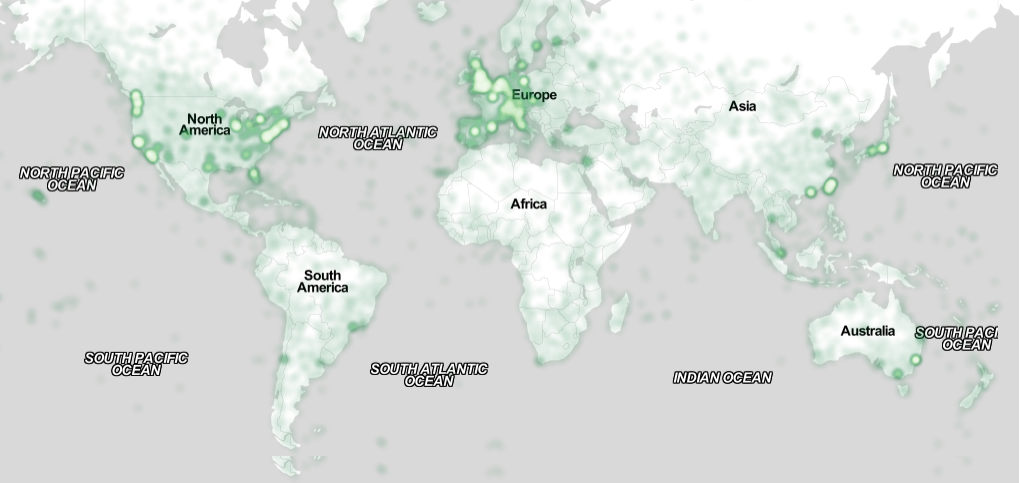
\includegraphics[width=\textwidth]{res/map}
\caption{A sample black and white graphic
that needs to span two columns of text.}
\end{figure*}


\begin{figure}

\includegraphics[height=1in, width=1in]{res/cats}
\caption{A sample black and white graphic that has
been resized with the \texttt{includegraphics} command.}
\end{figure}

\subsection{Theorem-like Constructs}

Other common constructs that may occur in your article are the forms
for logical constructs like theorems, axioms, corollaries and proofs.
ACM uses two types of these constructs:  theorem-like and
definition-like.

Here is a theorem:
\begin{theorem}
  Let $f$ be continuous on $[a,b]$.  If $G$ is
  an antiderivative for $f$ on $[a,b]$, then
  \begin{displaymath}
    \int^b_af(t)\,dt = G(b) - G(a).
  \end{displaymath}
\end{theorem}

Here is a definition:
\begin{definition}
  If $z$ is irrational, then by $e^z$ we mean the
  unique number that has
  logarithm $z$:
  \begin{displaymath}
    \log e^z = z.
  \end{displaymath}
\end{definition}

The pre-defined theorem-like constructs are \textbf{theorem},
\textbf{conjecture}, \textbf{proposition}, \textbf{lemma} and
\textbf{corollary}.  The pre-defined de\-fi\-ni\-ti\-on-like constructs are
\textbf{example} and \textbf{definition}.  You can add your own
constructs using the \textsl{amsthm} interface\footnote{\url{https://ctan.org/pkg/amsthm}}.  The
styles used in the \verb|\theoremstyle| command are \textbf{acmplain}
and \textbf{acmdefinition}.

Another construct is \textbf{proof}, for example,

\begin{proof}
  Suppose on the contrary there exists a real number $L$ such that
  \begin{displaymath}
    \lim_{x\rightarrow\infty} \frac{f(x)}{g(x)} = L.
  \end{displaymath}
  Then
  \begin{displaymath}
    l=\lim_{x\rightarrow c} f(x)
    = \lim_{x\rightarrow c}
    \left[ g{x} \cdot \frac{f(x)}{g(x)} \right ]
    = \lim_{x\rightarrow c} g(x) \cdot \lim_{x\rightarrow c}
    \frac{f(x)}{g(x)} = 0\cdot L = 0,
  \end{displaymath}
  which contradicts our assumption that $l\neq 0$.
\end{proof}

\section{Conclusions}
This paragraph will end the body of this sample document.
Remember that you might still have Acknowledgments or
Appendices; brief samples of these
follow.  There is still the Bibliography to deal with; and
we will make a disclaimer about that here: with the exception
of the reference to the \LaTeX\ book, the citations in
this paper are to articles which have nothing to
do with the present subject and are used as
examples only.
%\section{Conclusion}
The conclusion.

\printbibliography

\end{document}
